\subsection{Clauset-Newman-Moore greedy modularity maximization}
\begin{frame}[fragile]{Intuition}
The Clauset-Newman-Moore (CNM) greedy modularity maximization algorithm is a popular method used in community detection, a field of network analysis. It is designed to partition a given network into communities, where members of each community are more densely connected to each other compared to members of different communities. The CNM algorithm aims to maximize the modularity of the network, which is a measure of the quality of the community structure.

The CNM algorithm aims to maximize the modularity of the network, which is a measure of the quality of the community structure. The algorithm was proposed by Aaron Clauset, Mark Newman, and Cristopher Moore in 2004, and it has since become widely adopted due to its simplicity and effectiveness.

The CNM algorithm is agglomerative method and follows a greedy approach, iteratively merging and splitting communities to optimize the modularity score.

\begin{center}
    \begin{figure}[!htp]
    \centering
    \includegraphics[width=0.7 \textwidth]{CNM.png}
    \caption{Louvain Algorithm}
    \label{subsection}
\end{figure}
\end{center}
\end{frame}
\begin{frame}[fragile]{PseudoCode}
\resizebox{0.8\textwidth}{!}{%
\begin{algorithm}[H]
    \caption{Clauset-Newman-Moore (CNM) Algorithm}
    \SetAlgoLined
    \KwIn{Network graph}
    \KwOut{Community structure}
    Initialization: Assign each vertex to its own community\;
    
    Calculate the initial modularity value \( Q_{\text{initial}} \)\;
    
    \Repeat{no further improvement in modularity is possible}{
            \ForEach{pair of communities \( C_1 \) and \( C_2 \)}{
                Calculate the change in modularity \( \Delta Q \) by merging \( C_1 \) and \( C_2 \)\;
            }
        }
    
    Find the pair \( (C_1, C_2) \) with the maximum increase in modularity \( \Delta Q_{\text{max}} \)\;
    
    Merge communities \( C_1 \) and \( C_2 \)\;
    Update the modularity value \( Q \) by adding \( \Delta Q_{\text{max}} \)\;
    \Return{Community structure}
    \end{algorithm}
    
\end{frame}

\begin{frame}[fragile]{Pros and Cons}
    \paragraph{Pros}
    \begin{itemize}
        \item Ease of implementation: Modularity Maximization (MM) is conceptually simple and can be implemented with relative ease compared to other algorithms. Several open-source libraries and software packages readily implement MM, making it accessible to a wide range of users.
        \item Scalability: MM efficiently scales to handle large networks with millions of nodes and edges. This makes it suitable for analyzing real-world networks like social media graphs, citation networks, and protein-protein interaction networks.
    \end{itemize}
    \paragraph{Cons}
    \begin{itemize}
        \item Resolution limit: MM is sensitive to the resolution parameter, which controls the granularity of the detected communities. Choosing an appropriate resolution parameter can be challenging, as it can significantly impact the community structure. Small values tend to result in many small communities, while large values lead to a few large communities, potentially missing finer-grained structures.
        \item Merging similar clusters: MM can be biased towards merging similar clusters, even if they are not well-connected, to maximize the modularity score. This can lead to communities that are not cohesive or representative of the underlying network structure.
    \end{itemize}
\end{frame}
\subsection{Louvain}
\begin{frame}[fragile]{Intuition}
Louvain algorithm is a fast implementation of community detection\\
It is a hierarchical clustering algorithm that involves two phases: modularity optimization and community aggregation
\begin{center}
    \begin{figure}[!htp]
    \centering
    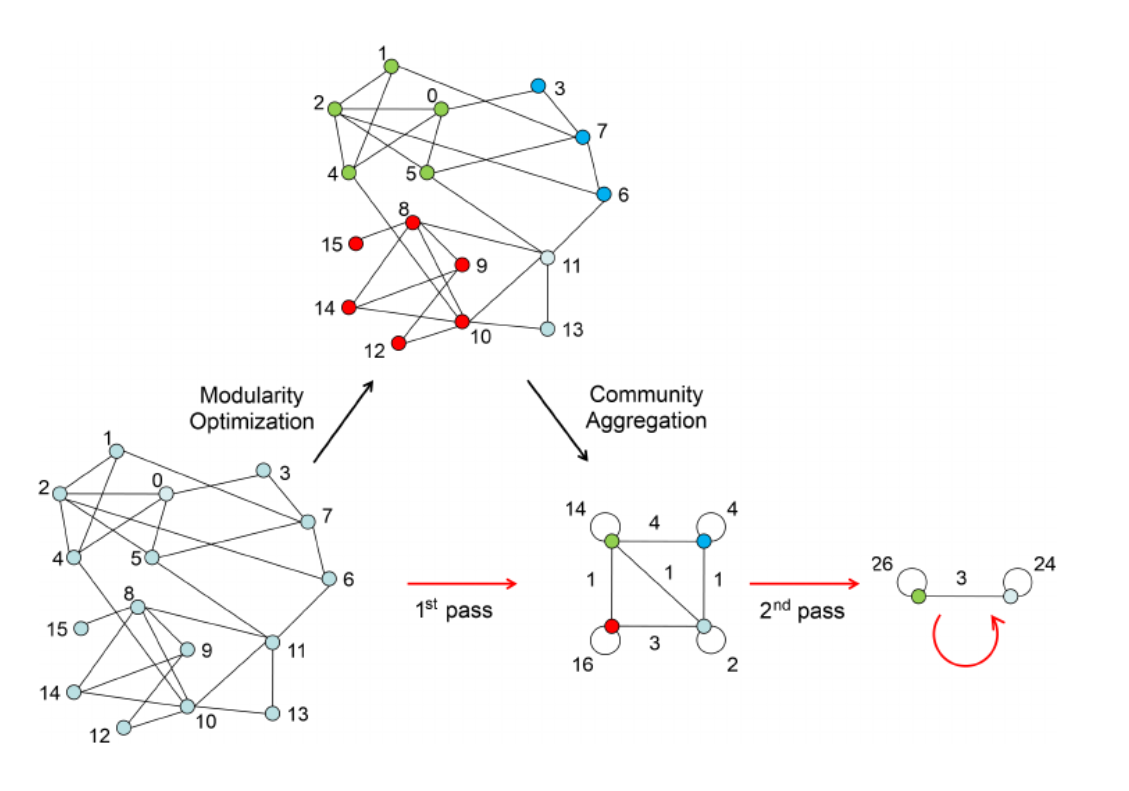
\includegraphics[width=0.7 \textwidth]{Louvain.png}
    \caption{Louvain Algorithm}
    \label{subsection}
\end{figure}
\end{center}
\end{frame}